\subsection{Kommunikationsprotokoll}\label{Protokoll}
\subsubsection{Projektteilbereich Übersicht}
Für die Kommunikation zwischen dem FPGA und dem UserInterface wurde ein spezielles Protokoll entwickelt, welches auf UART aufbaut. Ziel ist ein schnelles Senden der Messdaten und Austauschen der Konfiguration mit inkludierter Fehlerdetektion. Das gesamte Protokoll ist aufgebaut aus einzelnen Daten mit einer Wortlänge von 12-Bit, was die Handhabung der 12-Bit-ADC-Messwerte vereinfacht und praktisch für größere Zahlen ist, beispielsweise bei der Zeitbereichseinstellung (siehe: \ref{Zeitbereichseinstellung}). Es werden immer Pakete mit einem idententischen Aufbau gesendet.
\subsubsection{Paketspezifikation FPGA zu UserInterface}
\begin{figure}[!h]
\begin{center}
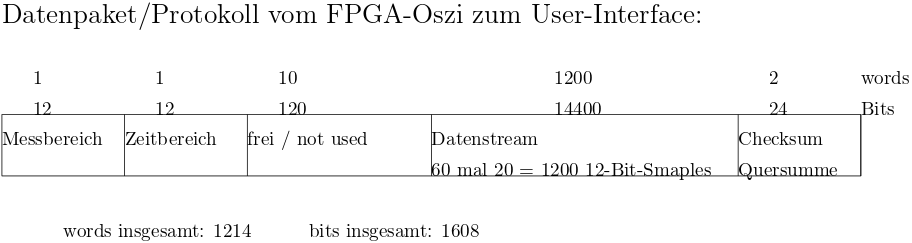
\includegraphics[width=15cm]{SAUER/Grafiken/Kommunikationsprotokoll/Datenstreampaket.png}
\caption{Paketspezifikation FPGA zu UserInterface}
\label{Datenstreampaket}
\end{center}
\end{figure}
\subsubsection{Paketspezifikation UserInterface zu FPGA}
\begin{figure}[h]
\begin{center}
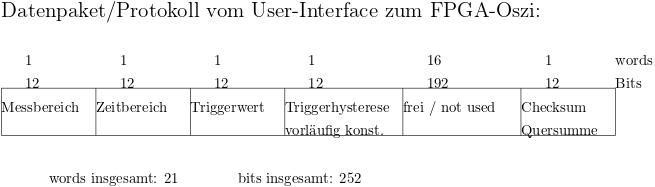
\includegraphics[width=15cm]{SAUER/Grafiken/Kommunikationsprotokoll/Controllerpaket.png}
\caption{Paketspezifikation UserInterface zu FPGA}
\label{Controllerpaket}
\end{center}
\end{figure}
\subsubsection{Messbereichseinstellung}
\subsubsection{Zeitbereichseinstellung}
\subsubsection{Messdaten}
\subsubsection{Checksum}
\subsubsection{frei / not used}
